\chapter{Алгоритмическое обеспечение и адаптация алгоритмов}

В этой главе рассматривается задача адаптации существующих алгоритмов,
используемых в различных системах АДТ для повышения производительности
процесса поиска логических выводов, \app{а также разработка других
специализированных алгоритмов}. Задача этой главы -- реализовать
полезные свойства ПО--исчислений при помощи известных мощных
алгоритмов поддержки различных этапов построения логических выводов. В
качестве таких алгоритмов выбраны \rem{...}{Можно перечислить имена,
  ссылки на литературу} В результате адаптации получены
\rem{...}{Что в результате получилось/удалось? }

%==========================================================
\section{Предпосылки разрабатываемых алгоритмов}

Для того что бы алгоритмы адекватно использовали возможности
ПО--формализма необходимо выявить его совместимые полезные свойства, а также свойства, не совместимые с адаптируемыми алгоритмами.  Полезные свойства представлены во введении и являются общепризнанными.

%--------------------ПРОБЛЕМЫ------------------------------------
\subsection{Проблемы формализма ПО-формул}
Укажем на некоторые свойства ПО-формализма, сказывающиеся на
\rem{производительности процесса поиска ЛВ и ...}{Как оно сказывается?} в частичном разрешении которых он нуждается.

\begin{enumerate}

\item Поиск ответов на вопросы с открытыми переменными требует выбора
  подставляемого терма для данной переменной из эрбранова универсума,
  который в общем случае, т.е. при наличии функциональных символов, является бесконечным множеством (счетным множеством). Какой именно терм необходимо выбрать --- изначально неизвестно.

Сделаем несколько замечаний. Во-первых, при решении прикладных задач, переменные связанные квантором всеобщности ограничиваются типовым условием, а значит появление открытых переменных в данном случае следует рассматривать как некую аномалию в следствии неверной формализации задачи. Это значит, что решение данной проблемы лежит вне прикладной области, и необходимо для решения общематематических теорем (например из библиотеки TPTP).  Во-вторых, есть соблазн уйти от функциональных символов (как это скромно сделано в \cite{Vas_ICDS}), но наличие функциональных символов есть основа сложных задач. В-третьих, в \cite{Vas_ICDS} предложена идея стратегии решения данной проблемы --- стратегия отсроченного присваивания (СОП), заключающаяся в том что изначально для открытой переменной выбирается неопределенный эрбранов элемент, а позднее он постепенно доопределяется. Подробное описание стратегии и её реализация представлены в главе 3. Данная стратегия конфликтует с другими стратегиями. Однако анализ решаемых задач показывает что в прикладных задачах (как-то их иначе наверное надо назвать) нет нужды использовать СОП ибо нет открытых переменных, а в общих задачах сложнее найти какие-то особенности которые применяются другими стратегиями, а значит конфликт частично разрешается просто разграничением областей применения системы.

\item Язык ПО-формул позиционируется как <<достаточно однородной, но в то же время хорошо структурированный>> и хорошо усваивающий эвристики. Стоит заметить, что однородность ПО-формул хуже чем, например, однородность дизъюнктов, в силу разнородных сущностей структуры формулы: база, вопросы, консеквенты вопросов. Разрешение данного вопроса требует применения специальных методов доступа к данным неоднородным частям.

\item Хотя изначально представление формулы ИП в языке ПО-формул более компактно чем КНФ, дальнейшее проведение правила вывода может привести к бОльшему усложнению структуры формулы (при наличии дизъюнктивного ветвления), чем при применении правила вывода в МР. Таким образом через некоторое количество шагов ввода размер ПО-формулы может оказаться в разы больше чем размер КНФ. Но эта проблема почти полностью устранима чисто техническими способами, а именно описанными далее методами разделения данных, а также ограничивающей стратегией (которую пользователь выбирает сам).

\end{enumerate}


%---------------------------
\subsection{Подходы}
Поскольку в данной работе рассматривается первопорядковый язык ПО-формул, некоторые из структур данных и алгоритмов имеют сходства с уже существующими системам АДТ первого порядка. Это касается структуры термов и подстановок. Кроме того существуют общетехнические методы независящие от конкретного формализма, например параллельные схемы алгоритмов, экономия потребляемой памяти, индексирование данных.

Таким образом в работе предполагается адаптация некоторых существующих алгоритмов, используемых в современных и самых эффективных системах АДТ. Адаптация предполагает, во-первых, учет особенностей ПО-формализма - как положительных так и проблемных, во-вторых, совмещение (синхронизация) алгоритмов, поскольку некоторые из них конфликтуют при прямой реализации.



%===============================================================
%---------------------------------------------------------------
%-----------------------АЛГОРИТМЫ---------------------------
\section{Алгоритмы и структуры данных}

%===================базовые структуры данных========================
\subsection{Общие структуры данных}

\textbf{Типы данных.} Язык представления формул имеет следующие типы данных: ATOM (атомарный символ), FUNCTION (функциональный символ), CONSTANT (константный символ), AVARIABLE (универсальная переменная), EVARIABLE (экзистенциальная переменная), UHE (Неопределённый Эрбрановский Элемент), INTEGER (целочисленный символ), FLOAT (нецелочисленный символ), STRING (строковый символ). Данные типы определяются перечислением:

{\tt enum SymbolType {CONSTANT, EVARIABLE, AVARIABLE, FUNCTION, ATOM, INTEGER, FLOAT, STRING, UHE};}


\textbf{Символ (Symbol).} Символ - буква из алфавита используемого языка. Структура Symbol содержит строковое представление символа, тип данных, арность. Символ идентифицируется по его адресу в памяти.

\textbf{Обобщённый терм (GTerm).} Такое название взято из \cite{NNN}. Смысл заключается в том что для представления как терма так и атома используется одна структура данных, поскольку и первые и вторые имеют древовидную структуру. Для правильной обработки соответствующих обобщенных термов используются вышеописанные типы данных. Терм представляется классической древовидной структурой каждый узел которой содержит символ верхнего уровня и массив ссылок на дочерние узлы. Универсальная переменная (AVARIABLE) и неопределённый эрбрановский элемент (UHE) используют один дочерний узел как ссылку на терм, который подставляется вместо данного. Если ссылка не UML значит переменная связана с некоторым термом. В противном случае переменная свободная для подстановки. Для того что бы корректно обрабатывать переменные, задан метод getValue() который возвращает значение типа GTerm. Если переменная не связана то значение getValue() совпадает со ссылкой на эту переменную, в противном случае возвращается ссылка на терм с которым связана переменная.

\textbf{Чанк.} Маркированный список. Список разделённый на подсписки любой длины (в том числе нулевой). Для каждого элемента списка можно определить к какому подсписку он относится. Далее будет показано что в каждом чанке хранится информация о текущем шаге выводе, а весь список в целом хранит всю информацию о формуле. Т.е. формула это список, а чанк это подформула полученная на определённом шаге вывода. На рисунке представлена структура чанкового списка.

\begin{figure}[h]
	%\vspace{0.5cm}
	\centering
	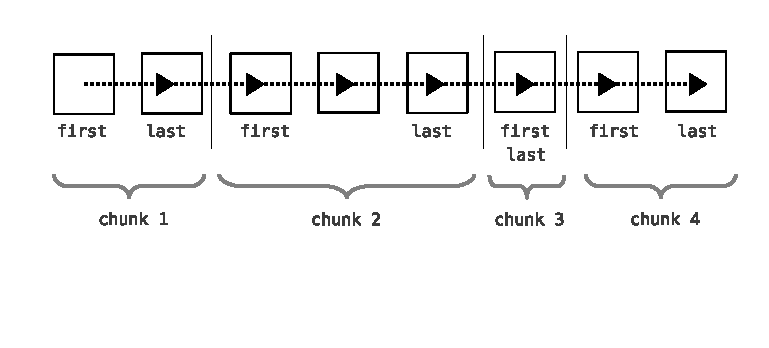
\includegraphics[width=0.6\linewidth]{pics/Chunk.eps}
	\caption{Чанковый список}
	\label{fig:chank1}
\end{figure}

На следующем рисунке показан случай когда один из чанков пуст.

\begin{figure}[h]
	%\vspace{0.5cm}
	\centering
	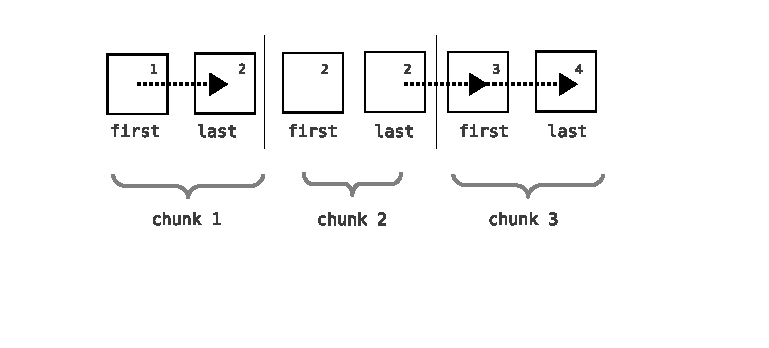
\includegraphics[width=0.6\linewidth]{pics/Chunk2.eps}
	\caption{Чанковый список}
	\label{fig:chank2}
\end{figure}

Стоп.


%=================== ДЕРЕВО СОСТОЯНИЙ ВЫВОДА =======================
\subsection{Дерево состояний вывода}
Одним из основополагающих методов в разработанной системе АДТ является дерево состояний вывода (ДСВ), состоящее из структур данных, характеризующих логический вывод и ряда методов, обрабатывающих данные структуры. Основная цель данного подхода заключается в том что бы строго зафиксировать все события произошедшие на каждом шагу логического вывода, например что бы точно определить какие данные были выведены на каком шагу вывода. Такая фиксация событий позволит:
\begin{enumerate}
 \item Более глубоко анализировать процесс ЛВ, а значит эффективно внедрять эвристики.
 \item Производить откаты в выводе (backtracking).
 \item Реализовать один из подходов разделения данных.
 \item Производить эффективное освобождение памяти.
\end{enumerate}

Для начала, кратко объясним идею ДСВ.
При классическом подходе после каждого ответа на вопрос к первоначальной формуле добавляется консеквент вопроса на который производился ответ (в базу добавляются соответствующие элементы узлов непосредственно следующих за вопросом; к вопросам добавляются новые вопросы, если они есть), а в случае дизъюнктивного ветвления соответствующая база расщепляется, не теряя никаких данных.
Таким образом, формула монотонно увеличивается, при этом сохраняя свою структуру.
ДСВ будем использовать для того что бы иметь полную информацию о текущей формуле, для возможности отката в выводе и подробного наблюдения за ним. Опишем ДСВ формально.

Дерево состояний вывода есть такое дерево, которое обладает следующими свойствами: корень дерева есть одна из базовых подформул первоначальной формулы; все остальные узлы есть добавляемые консеквенты (с примененным к ним подстановками-ответами и разыменованием переменных). Если приводить в пример определение правила вывода, то корень дерева это база E, а узлы это E2theta.
Таким образом если происходит расщепление то в данном узле появляется ветвление.
Отсюда можно говорить что каждая базовая подформула в формуле характеризуется соответствующим путём от листа до корня.

Как видно, каждый узел содержит самодостаточную информацию и для того чтоб производить откаты назад, достаточно удалять соответствующие узлы.
Кроме того такой подход реализует разделение данных (ссылок) на каждый консеквент, поскольку некоторые пути могут иметь общие подпути.
Если какая-то база опровергнута, то можно удалить все узлы от соответствующего листа до ближайшего ветвления, поскольку оставшаяся часть пути всё ещё используется для представления другой базы. Количество узлов равно текущему количеству баз. Если дерево пусто, значит первоначальная база опровергнута.
Та как изначальная формализация задачи в языке ПО-формул может содержать несколько базовых подформул, то для каждой из этих подформул строится своё ДСВ.

Для практических нужд узел ДСВ содержит некоторую системную информацию:
\begin{enumerate}
\item Множество атомов, понимаемых как часть базовых, отсюда каждый базовый конъюнкт характеризуется объединением всех множеств от данного узла до корня.
\item Список ссылок на вопросы к базе.
\item Для каждого вопроса определяется чанк ответов для вопроса в данный момент.
\item Номер последующего шага вывода и соответствующий ответ, если узел имеет потомков.
\item Чанк уже отработанных вопросов.
\end{enumerate}

Узлы содержат ещё различную информацию, которая будет описана ниже в описании стратегий вывода.

За счёт чанков получается разграничивать данные полученные на каждом шаге, с другой стороны на каждом шаге (в каждом узле) доступные все собранные до этого данные.

ДСВ для формулы из примера представлено на рисунке Рис.~\ref{fig:pst}.
Корнем ДСВ является первоначальная ПО-формула $F_1$. Узел ``2" является консеквентом вопроса $Q_1$, а именно $\exists\colon A(a)$, а путь от узла 2 до корня соответствует ПО-формуле $F_2$. Узлы 3 и 4 являются соответствующими консеквентами для вопроса $Q_4$. Путь от узла 3 до корня и путь от узла 4 до корня соответствуют базовым подформулам ПО-формулы $F_3$. Например, формулы определённые путями 5 --- 1 и 3 --- 1 разделяют данные которые представлены узлами 1 --- 2. Когда базовая подформула, которая представлена узлами пути 3 --- 1 опровергнута, то можно удалить путь от узла 3 до ближайшего ветвления (в сторону корня) --- в данном случае удаляется только узел 3, поскольку узлы 2 --- 1 всё ещё используются для представления других базовых подформул.

\begin{figure}[h]
	%\vspace{0.5cm}
	\centering
	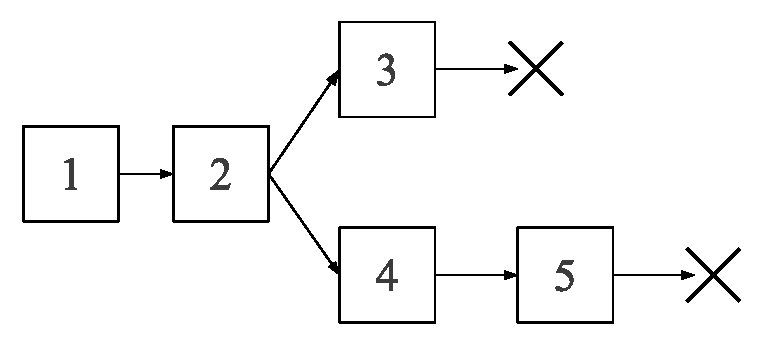
\includegraphics[width=0.4\linewidth]{pics/PST.eps}
	\caption{Дерево состояний вывода для формулы из примера \ref{proofexample}.}
	\label{fig:pst}
\end{figure}

На следующем рисунке представлено ДСВ с точки зрения его связи с чанками.

\begin{figure}[h]
	%\vspace{0.5cm}
	\centering
	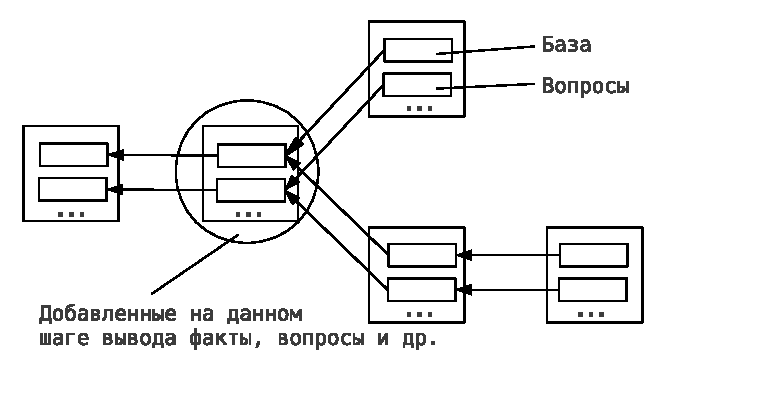
\includegraphics[width=0.6\linewidth]{pics/PST2.eps}
	\caption{ДСВ.}
	\label{fig:pst2}
\end{figure}

С точки зрения реализации ДСВ растёт от листов к корню.



%================================== СУПЕРВИЗОР =======================
\subsection{Супервизор}
Наблюдает глобально за всем деревом. Содержит информацию об ограничении ресурсов, эвристики и др.
В супервизоре находится список всех текущих листов дерева.
Большинство стратегий реализовано на уровне супервизора, поскольку иногда приходится читывать информацию о всей совокупности предшествующего или последующего вывода.

Наличие такого субъекта управления обусловлено тем что некоторые частные события в процессе логического вывода могут повлиять на него в целом.

%================================== ОГРАНИЧЕНИЕ РЕСУРСОВ =======================
\subsection{Стратегия ограниченных ресурсов.}
Стратегия ограниченных ресурсов есть в Вампире. У нас подобная стратегия напрямую зависит от текущего ДСВ и описывается так: ветка ДСВ строится до тех пор, пока не наступит ограничение разрешенной для использования памяти, либо пока не истечет определенное время, либо пока не будет произведено определенное количество шагов вывода. Если наступил предел использования ресурсов, то необходимо произвести откат назад и попробовать другие ответы, т.е. другие варианты построения дерева.

%============================================================================
%================================== РАЗДЕЛЕНИЕ ДАННЫХ =======================
\subsection{Разделение данных}
Логический вывод как правило связан с выводом новой информации. Например, в МР выводятся новые дизъюнкты до тех пор пока не выведется пустой, а в методе доказательства ПО-формул производится насыщение баз фактами до тех пор пока они не станут противоречивыми. Поскольку сложность формул может быть сколько угодно большой и даже минимальный вывод может иметь сколько угодно большую длину, имеет место быть проблема увеличения затрачиваемых ресурсов на всеразростающиеся формулы. Опыт показывает [ссылка] что автоматический вывод довольно быстро занимает всю имеющуюся в распоряжении память и далее процесс вывода требует регулярное удаление излишков. Таким образом проблема экономии памяти  довольно важна, особенно с учётом увеличения сложности задач. Для экономии памяти используются, во-первых проектирование компактных структур данных, во-вторых методы разделения общих участков памяти (data sharing). В случае логических языков и конкретно языка ПО-формул метод разделения данных довольно актуален.

Исходя из некоторых общих особенностей представления языков первого порядка и представления ПО-формул, нами выделено четыре вида разделения данных.

\paragraph{Агрессивное разделение термов.} Заключается в том, что разделяются общие участки оперативной памяти среди термов. Например, в термах $A(g(a,f(x)),h(c))$ и $B(k,g(a,f(x)))$, подтермы $g(a,f(x))$ являются общими и представляют собой один и тот же участок в памяти. Данный подход позволяет достаточно сильно экономить оперативную память при ограниченных ресурсах, однако требует дополнительное процессорное время на вычисление общих подтермов. Такой метод является общеупотребимым в системах АДТ, классически варианты реализации представлены в [].

\paragraph{Мягкое разделение термов.} Отличается от агрессивного намного большей эффективностью в смысле потребления процессорных ресурсов, но меньшей эффективностью с точки зрения экономии памяти, поскольку разделяет только часть общих подтермов. Опишем данный метод более подробно. Исходя из определения \ref{ircond} применение правила вывода $\omega$ законно в случае выполнения условия $A\theta \subseteq B$, где $A$ и $B$ соответственно конъюнкты вопроса и базы. Поскольку $B$ это уже существующее множество основных обобщенных термов, то для их хранения выделена соответствующая память. $\theta$ же является отображением переменных вопроса $A$ в элементы эрбранова универсума. В дальнейшем при применении правила вывода $\theta$ применяется ко всему консеквенту вопроса и данный консеквент добавляется к формуле. Однако правая часть подстановки уже имеется в памяти, в силу того что основана она на $B$. Исходя из этого достаточно использовать ссылки на уже имеющуюся память используемую для правых частей подстановки в тех частях консеквента где эта подстановка применяется. На рисунке детально представлена данная ситуация.

\paragraph{Разделение базовых подформул.} ПО-формулы, в которых производится ответ на вопрос имеющий вопрос с дизъюнктивным ветвлением, расщепляются на несколько новых базовых подформул. Количество новых базовых подформул совпадает с количеством непосредственных наследников в консеквенте вопроса. В прямом варианте такое расщепление требует копирования предыдущего состояния формулы несколько раз, такое копирование естественно приводит к большим затратам памяти и процессорному времени предназначеннго для копирования. Решение данного вопроса могло бы лежать в плоскости агрессивного разделения термов, однако такого разделения может быть недостаточно. Если формула предполагает достаточно сильное ветвление, сохраняется проблема наличия множества ссылок на разделяемые атомы баз. Поскольку расщепление предполагает разделение баз, то имеет смысл разделять и эти ссылки. Более подробно ситуация рассмотрена на рисунке.

Таким образом в системе кроме разделения термов используется ещё и разделение ссылок на эти термы, благодаря ДСВ.

\paragraph{Разделение переменных и неопределенных эрбрановских элементов.} Предназначено для быстрого применения подстановки ко всей формуле, т.к. все одноименные переменные в формуле представляют собой один участок в памяти. О неопределенных эрбрановских элементах сказано ниже. Все одноименные переменные на протяжении любого основного пути формулы \cite{dissChe} являются указателем на один и тот же участок в памяти. В отличие от агрессивного разделения данный подход учитывает роль переменных в процессе поиска ответных подстановок. В процессе применения подстановки переменная не заменяется на терм, а лишь указывает на этот терм, что позволяет экономить время на замену переменной термом в поддереве.

\paragraph{Веса подформул.} Кроме непосредственно экономии потребляемой памяти, реализована возможность сдерживания разрастания формулы. Для этого из возможных ответов на вопрос выбирает тот который приводит к формуле наименьшего веса. Под весом понимается количество узлов в дереве представляющем терм или формулу.


%======================== INDEXING ===========================
\subsection{Индексирование данных}

Из определения стратегии ясно, что шаг вывода зависит от некоторых \textbf{критериев}, которым должны удовлетворять определенные части ПО-формулы. Например, допустимы следующие критерии: Наличие в базе заданного терма, наличие вопроса с заданными свойствами, количество вхождений терма в конъюнкт и т.д. Для определения истинности данных критериев необходимо проводить поиск и анализ данных в формуле. С каждым шагом вывода формула в общем случае увеличивается (причем в некоторых случаях довольно сильно), и может настать момент когда поиск тех или иных данных будет затруднен.

%индексирование термов
\paragraph{Индексирование термов}

В информационных технологиях подобные проблемы разрешены с помощью методов индексирования данных (широкоприменяемых в базах данных \cite{Ulman}). Подобно тому как в библиотеке книги проиндексированы первыми буквами своих названий а также именами авторов. Такие подходы используются и в реляционных БД.

В нашем случае основной объект индексирования есть терм, который является древовидной структурой, индексирование которой в реляционных БД неэффективно [есть ссылка на это]. Поэтому следует использовать иные подходы.

Индексирование термов --- хорошо исследованный вопрос, как в рамках определенных систем АДТ, так и абстрактно. В частности по данной теме можно почитать [дискриминационное дерево и пути, подстановочное дерево, и книжку Графа про индексирование].
Перечисленные методы, позволяют эффективно находить в базе термов те термы, которые удовлетворяют определенным критериям: являются равными данному (query term), являются его примерами, обобщениями (generalization) и унификациями.
Для наших нужд не требуется обобщение и классическая унификация, но дополнительно необходимы НЭЭ Унификация, критерий наличия термов включающих заданный подтерм, и различные количественные критерии: вес, глубина, арность. С учетом перечисленных требований а также того факта, что как правило в базе находятся основные термы, мы в качестве основы выбрали методику индексирования путями [].

Кратко опишем её суть, как она описана в []. Для каждого атома составляется список так называемых путей. [Надо привести формальное определение пути из [макКьюн]]. Например, атом $A(g(x,c),e)$ представляется в виде путей $A$, $A1g$, $A1g1x$, $A1g2c$, $A2e$. Каждый из этих путей содержит указатель на соответствующей атом. Сами пути хранятся в отсортированном виде (в дереве).

Пример. Пусть дан атом $A(a,f(x,b))$ и множество атомов $\{A(a,f(c,b)), A(a,f(b,e)),A(a,f(k,b)), A(b,f(e,b))\}$. Любой атом, являющийся основным примером для заданного, содержит в своём списке путей следующие пути: $A1a$, $A2f2b$. Таким образом для поиска основных примеров заданного атома необходимо найти пересечение множеств атомов, на которые указывают пути.  В частности путь $A1a$ указывает на множество $\{A(a,f(c,b)), A(a,f(b,e)),A(a,f(k,b))\}$, а путь $A2f2b$ на $\{A(a,f(c,b)), A(a,f(k,b)), A(b,f(e,b))\}$. Пересечение этих множеств есть множество $\{A(a,f(c,b)),A(a,f(k,b))\}$, это и есть множество примеров для атома $A(a,f(x,b))$.

Заметим, что методы индексирования термов на сегодняшний день используются во многих известных системах АДТ [Vampire -улучшенное индексирование путями, Otter -дискр.дерево и пути, E, EQP, SPASS -дерево подстановок].

Кроме базы термов, в индексировании нуждаются множества вопросов и множества ответных подстановок.

%индексирование других частей фомрулы
\paragraph{Индексирование других частей формулы}
Теперь опишем иные нужды индексирования. Предположим что у нас имеется некоторая стратегия для решения некоторого класса задач. Стратегия оперирует вопросами с определенными свойствами (т.е. вопросу сопоставляется содержательная информация), которые присущи всему классу задач (т.е. все задачи объединяет наличие определенных вопросов).
Естественно было бы неплохо как-то закрепить эти вопросы что бы упростить в дальнейшем к ним доступ и каждый раз не проверять все вопросы на наличие определенного свойства.
Для этого достаточно сделать словарь (map) в котором каждому описанию вопроса соответствовал бы указатель на данный вопрос. (Конечно можно в стратегии пользоваться лишь номером вопроса, но тогда теряется гибкость, ведь пользователю необходимо будет ставить вопросы всегда на одно и тоже место.)
Данный вид индексирования (весьма простого) может выполняться как на этапе компиляции (тогда в компиляции прувера будет задействован не только стратегия но и сама задача), так и при первичном обращении к вопросу (тогда нет необходимости в компилировании самой задачи).


%================================== ЛЕНИВАЯ КОНКРЕТИЗАЦИЯ =======================
\subsection{Неограниченные переменные}
Проблема неограниченных переменных описана выше. Для её решения предложено несколько подходов.

\paragraph{Ленивая конкретизация}
Суть заключается в следующем: для открытой переменной не выбирается конкретный элемент эрбранова универсума, а в место этого она заменяется на неопределенный эрбрановский элемент (НЭЭ), который в дальнейшем исходя из нужд вывода постепенно доопределяется до основного терма, либо в некоторых ситуациях так и остается недоопределенным.
По своей природе НЭЭ схож с переменной в том смысле что он изменяем, однако все изменения касающиеся НЭЭ должны быть направлены на конкретизированные НЭЭ, т.е. НЭЭ может быть заменен либо на некий терм (возможно тоже содержащий НЭЭ) либо на другой НЭЭ, но не на переменную. Однако для переменной НЭЭ считается как терм, и можно производить замену на него.

\begin{equation}
	\forall\colon\boldsymbol{True} - \exists\colon\boldsymbol{True} -
	\left\lbrace
	\begin{array}{l}
		\forall x\colon\boldsymbol{True} - \exists\colon A(x) \\
		\forall x\colon A(f(x)) - \exists\colon B(f(x)) \\
		\forall\colon B(f(a)) - \exists\colon \boldsymbol{False}
	\end{array}\right.
\end{equation}
На первом шаге вывода имеется ответ $\{x \rightarrow h_1\}$ на первый вопрос, $x$ является неограниченной переменной, $h_1$ это неопределённый эрбрановский элемент (НЭЭ). После первого шага атом $A(h_1)$ Добавляется в базу. На втором шаге вывода имеется ответ $\{x \rightarrow h_2\}$ на второй вопрос, и $h_1$ конкретизируется до $f(h_2)$, после второго шага $B(f(h_2))$ добавляется в базу. Наконец, на третьем шаге имеется тривиальный ответ на третий вопрос и $h_2$ доопределяется до $a$.

Однако существуют особые ситуации. Рассмотрим следующий пример:
$$\fictAquantor \; - \; \exists\colon M(e) \left\{
\begin{array}{lcl}
 \forall x,y\colon M(x) & - & \exists\colon S(y),M(f(x)),T(x) \\
 \forall x \colon T(x),S(e) & - & \exists\colon Q(x) \\
 \forall x \colon Q(x),S(f(e)) & - & \exists\colon\textbf{False}
\end{array}
\right.$$

Данная формула имеет вывод, например такой: отвечаем на первый вопрос с подстановкой $\{ x\rightarrow e, y\rightarrow e \}$, в результате в базу попадают факты $S(e),M(f(e)),T(e)$; ответ на второй вопрос есть $\{ x \rightarrow e\}$ и в базу попадает $Q(e)$; полученных фактов в базе недостаточно для ответа на целевой вопрос, поэтому вновь отвечаем на первый вопрос, при этом имеет несколько вариантов ответа, но важно переменную $y$ необходимо заменить на $f(e)$, выберем, например, следующий ответ $\{x \rightarrow e, y \rightarrow f(e) \}$ и в базу попадет факт $S(f(e))$ после чего целевой вопрос имеет ответ.
Заметим что на первый вопрос необходимо обязательно выбирать те подстановки которые содержат $y \rightarrow e$ и $y \rightarrow f(e)$ необходимые для ответа на второй и третий вопросы соответственно. Также формула устроена таким образом что первый и второй вопросы всегда имеют новые ответы (надеюсь это очевидно).

Теперь рассмотрим работу стратегии отсроченного присваивания: ответ на первый вопрос будет следующего вида $\{ x\rightarrow e, y\rightarrow h_1 \}$, где $h_1$ есть НЭЭ, и в базу попадают следующие факты $S(h_1),M(f(e)),T(e)$; ответ на второй вопрос есть $\{ x\rightarrow e, h_1\rightarrow e \}$ в котором $h_1$ доопределяется до $e$ и соответственно находящийся в базе факт $S(h_1)$ доопределяется до $S(e)$; с этого момента начинается зацикливание, поскольку целевой вопрос не имеет ответа, вновь отвечаем на первый вопрос и вновь в базу попадает факт $S(h_1)$, который при ответе на второй вопрос вновь доопределится до $S(e)$ и т.д. Однако если пропустить ответ на второй вопрос, то при ответе на целевой, факт $S(h_1)$ доопределится до $S(f(e))$ и на этом вывод закончится.

В общем виде проблема заключается в том, что НЭЭ доопределяется при поиске ответов на определенный вопрос, раньше чем это необходимо при ответе на другой вопрос. То есть доопределяется там где этого уже не надо.

Из подобных примеров видно, что СОП не может использоваться на прямую. Необходимы какие-то дополнительные средства обеспечения логического вывода.

\paragraph{Первый вариант}
Одним из вариантов решения проблемы является использование языка описания стратегий, с помощью которого можно, например, указать, что на второй вопрос необходимо ответить лишь один раз, либо использовать на первый вопрос сразу несколько подстановок содержащих $y\rightarrow h_1$ и $y\rightarrow h_2$, это приведет к попаданию в базу двух фактов $S(h_1)$ и $S(h_2)$, один которых будет использоваться для второго вопроса, а другой для целевого. Такой вариант вполне приемлем и нами предполагается что именно он и будет чаще всего использоваться для решения задач. Но что делать, если дополнительные знания о задаче не позволяют сформулировать правильную стратегию? Необходимо предоставить хотя бы принципиальную возможность вывода (что пока необеспеченно).

\paragraph{Второй вариант}
Мы видим следующий путь решения данной проблемы в общем случае (т.е. без использования дополнительных стратегий): не доопределять НЭЭ на месте (как это сделано выше), а \textbf{порождать} новые выражения, полученные из исходных, заменой в них НЭЭ на доопределение. То есть если в базе содержится факт $S(h_1)$ и $h_1$ необходимо доопределить до некоторого терма $t$, то в базу добавляется новый факт $S(t)$, порожденный от $S(h_1)$, при этом сам $S(h_1)$ сохраняется. При определенных условиях также может возникнуть ситуация когда будут порождаться не только факты, но и целые подформулы.
Содержательно такой подход означает следующее: можно считать что для вопроса с открытыми переменными применяется вся совокупность возможных ответов (с использованием всех элементов эрбрановского универсума), но так как технически это нереализуемо (из-за бесконечности эрбановского универсума), используется техника ленивых вычислений. В уме мы думаем что применили все ответы, а на деле используем только необходимые.

Данный подход имеет и определенные недостатки. Связано с тем если появится вопрос с НЭЭ, то придется порождать новые вопросы, а если будет диз.ветвление, то ещё хуже. Плюс во время унификации вылазят всякие проблемы. Короче об этом надо упомянуть но сильно не выпячивать, и оправдаться тем что мы больше нацелены на использование миниязычка, а эта стратегия дана лишь для обеспечения полноты вывода. Но эта стратегия вполне эффективна если НЭЭ не будут появляться новые вопросы с НЭЭ и в диз.ветвлении их не будет...

Отметим, что стратегии основанные на использовании НЭЭ стоят особняком для многих других стратегий. Во-первых из-за этой стратегии нарушается независимость базовых подформул, поскольку один и тот же НЭЭ может быть в разных подформулах, то доопределение одного из них в одной подформуле автоматически приводит к доопределению его в другой подформуле, это в частности противоречит параллельным стратегиям и противоречит некоторым эвристическим фишкам.

\paragraph{Стратегия фильтрации эрбрановского универсума}
Ещё одним вариантом решения проблемы открытых переменных является стратегия фильтрации ЭУ. Данная стратегия позволяет избавиться от проблем вышеперечисленных, но несколько расширяет пространство возможных ответов. Суть данной стратегии заключается в следующем. Атомы консеквентов, которые (атомы) содержат неограниченные переменные вопросов, должны унифицироваться с одноимёнными атомами из всех других частей всей базовой подформулы, в противном случае атом попавший в базу не будет удовлетворять условие применения правила вывода, поскольку никода не выполнится процедура матчинга при поиске ответов. Будем использовать данное свойство в стратегии. В качестве ответа для неограниченных переменных используются основные примеры унификации. Такой подход позволяет заранее сузить пространство ЭУ, фильтруя заведомо бесполезные ответы.

Для ясности рассмотрим пример.



%======================================================================
%================================== k,m-условие =======================
\subsection{Стратегия km-условия}
Данная стратегия формулируется следующим образом. Некоторый ответ применяется, если за последующие k шагов произойдет заданное событие m раз. Пользуясь терминологией ДСВ это означает что для данного узла дерева применяется ответ в случае если построенное в результате дальнейшего вывода поддерево коренящееся с этого узла не превысит глубину k и до этого момента произойдет m раз событие.

Мы предлагаем три спецификации данной стратегии.

\textbf{km-опровержение.} Ответ выбирается в случае если за последующие k шагов будет опровергнуто m баз. Подобная стратегия первоначально предложена в \cite{ICDS2000} и реализована в КВАНТе Черкашина. В данной системе эта стратегия расширена вторым параметром m. Она позволяет сдерживать разрастание пространства поиска вывода, т.е., сдерживает излишнее ветвление ДСВ, что в некоторых случаях приводит к многократному усложнению вывода.

\textbf{km-конкретизация.} Если за последующие k шагов будет доопределено m НЭЭ. Эта стратегия также направлена на то чтоб ограничить сложность представляемой формулы. Недоопределенный НЭЭ тащит много информации за собой и много условий, что на уровне реализации влияет негативно, поэтому чем больше и быстрее НЭЭ будут доопределены нужным образом, тем лучше.

\paragraph{Особенности реализации}
Основной для реализации данной стратегии являются описанные выше ДСВ и супервизор. Параметры k,m и собственно условие закладывается в супервизоре и привязывается к определённом узлу ДСВ. Через каждый следующий шаг вывода, супервизор проверяет все условия. И в положительном случае производится откат назад, т.е. последовательное удаление узлов дерево в обратном порядке (от листа в направлении корня). Перед удалением каждого узла производится разконкретизация НЭЭ полученных на этих узлах и возврат использованных вопросов в стадию активных (т.е. возможных для применения).

%================================== КЕШИРОВАНИЕ =======================
\subsection{Кэширование результатов}
Учитывая множественность возможных ответов, откатов в выводе, большой глубины вывода, большого количества атомов в базе и т.д. целесообразно кешировать некоторые результаты чтобы не производить снова повторяющиеся вычисления.

Добавление уже имеющихся в базе атомов не допускается. Поэтому процедура поиска ответов работает всегда с новыми атомами, и производит всегда новые вычисления. Тем не менее полученные ответы в итоге могут совпадать. Все примененные ответы сохраняются, причем хранятся они как и база в чанках, размазанных по всему пути от листа до узла. Это позволяет делать корректные откаты с учетом сохранения информации о примененных ответах.

%-----------PARALLEL STRATEGY---------------------------
\subsection{Параллельные стратегии}

Полезно сполна использовать все вычислительные ресурсы. Многие современные ВС обладают бОльшим чем 1 вычислительным элементом (процессором).

Предлагаем следующие стратегии для распараллеливания процесса логического вывода.

\paragraph{Первая стратегия}

В случае если вопрос имеет дизъюнктивное ветвление, то после ответа на этот вопрос, формула расщепляется и трансформируется в формулу с б'ольшим количеством баз. Таким образом, количество базовых подформул может заметно увеличиваться. Кроме того, исходная формализация задачи в языке по-формул может содержать более одной базовой подформулы. Для того, что бы показать, что исходная формула противоречива, необходимо опровергнуть каждую из баз. Специфика исчисления ПО-формул, позволяет рассматривать данные базы независимо друг от друга (естественный ИЛИ-параллелизм, следующий из того что в базах находятся лишь основные термы), а значит, процедура опровержения каждой базы может выполняться в отдельном вычислительном процессе. Таким образом, первая стратегия, реализуемая в виде параллельной схемы алгоритмов, формулируется следующим образом: каждая базовая подформула опровергается независимо, а значит параллельно. Для нужд данной стратегии как раз и реализовано жесткое копирование (следующая глава), что бы полностью скопировать базовую подформулу и обрабатывать её в отдельном процессе независимо (не разделяя память).

\paragraph{Вторая стратегия}
Для применения каждого шага логического вывода, необходимо выполнять, в общем случае, поиск ответных подстановок для заданного вопроса. Поиск ответных подстановок не изменяет структуру формулы, и не использует общих изменяемых данных, это значит, что процессы поиска ответа на каждый вопрос независимы, а значит параллельны.


\paragraph{Третья стратегия}
Теперь рассмотрим процедуру поиска подстановок для отдельно взятого вопроса.
Как было сказано во введении, подстановка $\theta$ является ответом, если выполняется
условие $A\theta \subseteq B$, где $B$ --- конъюнкт вопроса, $A$ --- конъюнкт базы.
Для сохранения полноты необходимо хотя бы потенциально иметь в распоряжении все возможные ответы,
из которых выбирается подстановка для данного шага. Ниже описан структура хранилища ответов. Можно говорить о том что наполнение каждого чанка хранилища подстановками производится параллельно, поскольку чанки независимы.

\paragraph{Свойства стратегий}

Анализ, описанных выше стратегий, показывает, что они обладают свойством вложенности. Т.е., для того, что бы опровергнуть одну базовую подформулу (первая стратегия) необходимо найти ответы на вопросы (вторая стратегия). В свою очередь для поиска ответа, необходимо найти подстановки для каждого атома из конъюнкта вопроса (третья стратегия).

Исходя из этого, данные стратегии можно разместить по степени эффективности (иерархия стратегий). Не трудно видеть, что время, затрачиваемое на опровержение базы, как минимум, не меньше, чем время, затрачиваемое на поиск ответных подстановок, а на практике, как правило, оказывается намного больше (так как, как правило, для опровержения базы необходимо неоднократно ответить на некоторые вопросы). Аналогичные выводы делаются по отношению к другим стратегиям.

Кроме того, можно выделить единое для всех стратегий свойство – свойство однородности. Т.е. стратегии имеют единую структуру. А именно, все они, по сути, сводятся к применению некоторой операции (опровержение базы, поиск ответов и т.д.) для каждого элемента некоторого множества (базы, вопросы и т.д.).

Одной из рекомендаций при реализации описанных алгоритмов на кластерных вычислительных системах является правильное распределение задач между вычислительными узлами кластера, в зависимости от скорости коммуникации между ними. Например, программная реализация первой стратегии должна процесс привязывать к вычислительному узлу. Однако этого не стоит делать при реализации остальных стратегий, так как коммуникационные затраты, вполне вероятно, перекроют полезное время вычислений, и тем самым лишь ухудшат результат.

Отметим что данная стратегия в общем случае конфликтует со стратегией отсроченного присваивания (поскольку СОП может нарушать независимость баз и вопросов).

\paragraph{Тестирование}
Важным свойством параллельных схем алгоритмов является их масштабируемость, т.е. степень повышения эффективности с увеличением количества вычислительных элементов (ВЭ). Поэтому основной характеристикой является не конкретное время исполнения программ, а соотношение времени исполнения программы в параллельном режиме на заданном количестве ВЭ к времени исполнения этой же программы на одном ВЭ при различном количестве ВЭ.

Эксперименты проводились на задачах, формализация которых в языке ПО-формул обладает необходимыми свойствами для испытания параллельных стратегий, а именно: дизъюнктивное ветвление, большое количество вопросов, крупные конъюнкты вопроса.

Результаты находятся в соответствии с представленной иерархией стратегий. На рис. представлены результаты тестирования.

\begin{figure}[h]
	%\vspace{0.5cm}
	\centering
	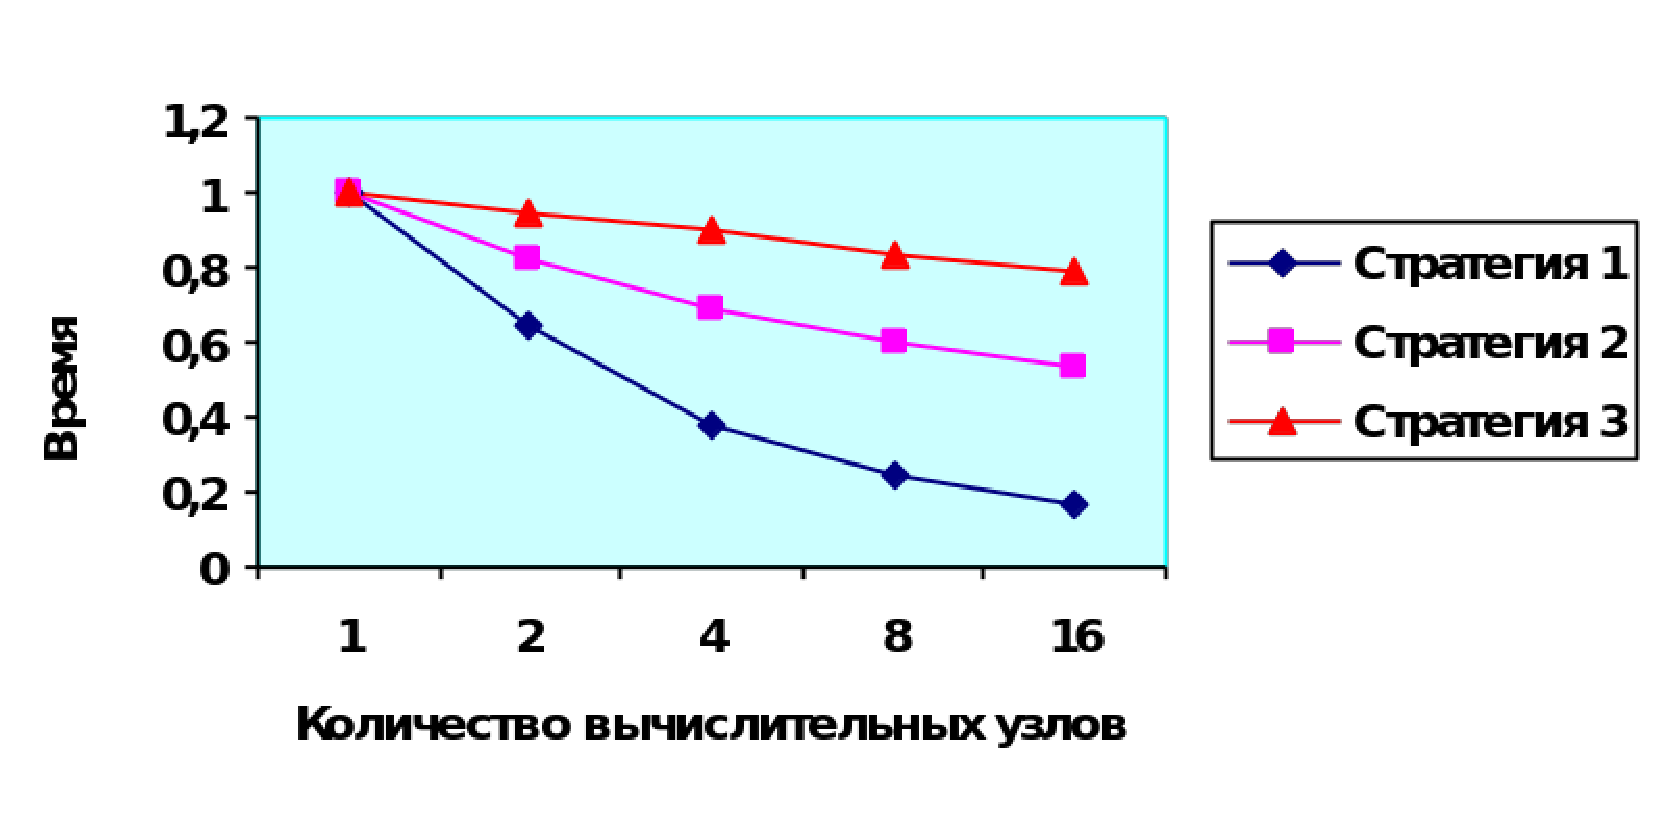
\includegraphics[width=0.6\linewidth]{pics/Parallel.eps}
	\caption{Параллельные стратегии}
	\label{fig:parallel}
\end{figure}

Наибольшую эффективность, как и следовало ожидать, показала первая стратегия (естественно при наличии дизъюнктивного ветвления). Под эффективностью понимается уменьшение затрачиваемого времени с увеличением количества вычислительных узлов.


%============================= РАВЕНСТВА =========================
\subsection{Равенства}
Для работы с равенствами как правило очень неэффективно напрямую использовать аксиомы равенства (рефлексивность, симметричность, транзитивность, подстановочность). Например, если формула содержит лишь один бинарный функциональный символ $f$ и один бинарный атомарный символ $A$, то в языке ПОФ аксиомы равенства для такой формулы будут представлены следующим образом:
$$\left\lbrace
\begin{array}{l}
\forall x\colon\boldsymbol{True} - \exists\colon x = x \\
\forall x_1,y_1,x_2,_y2\colon x_1 = y_1, x_2 = y_2 - \exists\colon f(x_1,y_1) = f(x_2, y_2) \\
\forall x_1,y_1,x_2,_y2\colon x_1 = y_1, x_2 = y_2, A(x_1,y_1) - \exists\colon A(x_2,y_2)
\end{array}\right.
$$
Таким образом, для каждого функционального и атомарного символа из формулы ставится в соответствие подформула-вопрос аксиома равенства. Явное использование таких аксиом во-первых, усложняет структуру формулы (лишние вопросы), во-вторых, увеличивает число шагов вывода, в-третьих, генерирует много (потенциально бесконечно) фактов в базе, возможно ненужных, мешающих выводу.

Отметим что данная проблема не так ужасна как в МР, поскольку в МР могут генерироваться лишние дизъюнкты, а это соответствует генерированию лишних вопросов в ПОФ. В исчислении ПОФ же генерируются лишь атомы-факты, за которыми проще наблюдать, но тем не менее их много.

При классическом подходе, в соответствии с определением ~\ref{ircond} подстановка $\theta$ является ответом на вопрос, тогда и только тогда, когда $A \theta \subseteq B$ где $A$ - конъюнкт вопроса, а $B$ - конъюнкт базы. Поиск ответов есть задача поглощения, для решения которой как правило используется алгоритм матчинга, об этом уже писалось выше. В случае ПОФ используется основной матчинг, а в случае НЭЭ используется полуосновной-матчинг.

Для решения проблемы основного матчинга без явного использования аксиом равенства имеется задача основного матчинга с равенствами, которая формулируется следующим образом [microsoft]:
Для данного множества равенств $E(B)$, основного терма $t$ и терма $p$, который может содержать переменные, необходимо найти множество подстановок $\theta$, по модулю $E(B)$, такие что $E(B)\models t = p\theta$. Через $E(B)$ мы обозначим множество всех равенств в данной базе $B$. Две подстановки эквивалентны если их правые части попарно конгруэнты по модулю $E(B)$.

Для поиска таких ответов мы используем аппарат теории систем переписывания термов \cite{Nipkow}.



%=====================================================================
%==========================ХРАНИЛИЩЕ ОТВЕТОВ==========================
\subsection{Хранилище ответов}
Хранилище ответов предназначено для эффективной организации работы с ответными подстановками и синхронизации с бэктрэкингом.

Каждому атому конъюнкта вопроса соответствует чанк возможных подстановок, матчащих этот атом с атомами из базы. Использование чанков связано с тем что необходимо точно определять на каком шаге какие подстановки были найдены. Для поиска ответа на вопрос, необходимо учитывать совокупность чанков соответствующих всем атомам конъюнкта вопроса.

На рисунке представлена схема хранения подстановок.

\begin{figure}[h]
	%\vspace{0.5cm}
	\centering
	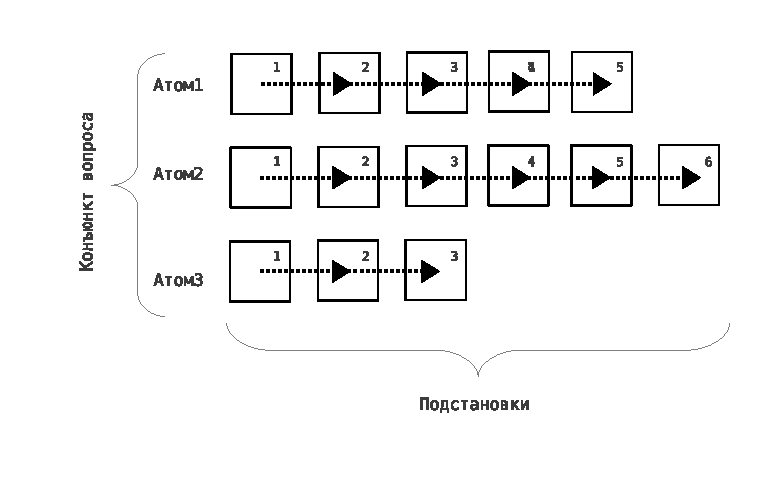
\includegraphics[width=0.6\linewidth]{pics/AnBase.eps}
	\caption{Подстановки}
	\label{fig:anbase}
\end{figure}

Далее из этой структуры выделяется ответ на вопрос. Для этого комбинируются подстановки из каждого чанка по одной. При этом подстановки должны быть совместимы. Две подстановки совместимы если их левые части равны, а правые унифицируемы. Например, если есть подстановки $\{x \rightarrow a\}$ и $\{x \rightarrow b\}$, где $b$ есть константа, то эти подстановки несовместимы, поскольку $a$ и $b$ неунифицируемы. А подстановки $\{x \rightarrow f(a)\}$ и $\{x \rightarrow f(h)\}$, где $h$ есть НЭЭ, совместимы, поскольку $f(a)$ и $f(h)$ унифицируемы с подстановкой $\{h \rightarrow a\}$. Результатом комбинации будет объединение всех совместимых и унифицирующих подстановок.

Перебор подстановок из чанков производится последовательно, это позволяет сохранить полноту.

%=================================================================================
%==================================СТАНДАРТНАЯ СТРАТЕГИЯ==========================
%=================================================================================
\subsection{Стандартная стратегия}
Главное свойство стандартной стратегии заключается в её полноте. Для полноты вывода необходимо организовать полный последовательный перебор всевозможных ответов на все вопросы. Для этого используются возможности дерева состояний вывода и хранилища ответов.


%%% Local Variables:
%%% mode: latex
%%% TeX-master: "dis"
%%% End:
